\documentclass[12pt]{article}
\usepackage{amsmath}
\usepackage{amssymb}
\usepackage{amsthm}
\usepackage{cancel}
\usepackage{enumitem}
\usepackage{esdiff}
\usepackage{graphicx}
\usepackage[version=4,textfontname=sffamily,mathfontname=mathsf]{mhchem}
\usepackage{multicol}
\usepackage{siunitx}
\usepackage{ulem}
% \usepackage{pgfplots}
\usepackage{wrapfig}
\usepackage{xcolor}

\newcommand{\e}[1]{e^{#1}}
\newcommand{\ei}[1]{e^{i\left(#1\right)}}
\newcommand{\E}[1]{\times 10^{#1}}
\newcommand{\tagref}[1]{\tag{\ref{#1}}}

\renewcommand\qedsymbol{TENA}

\title{
    Homework \#10
    \\  \small
    PHYS 4D: Modern Physics
    \\
    Problems from Krane's textbook
    }
\author{Donald Aingworth IV}
\date{March 23, 2026}

\begin{document}
\maketitle
\DeclareSIUnit{\amu}{amu}

\section{Chapter 9}
    \subsection{Question 1}
        Why does \ce{H2} have a smaller radius and a greater binding energy than \ce{H+2}?

        \subsubsection{Answer}
            A second electron being added to the \ce{H2+} to form \ce{H2} increases the electron density in between the two protons. 
            This pulls the two protons closer to the electrons and closer to each other. 
            It also amplifies the bonding energy since both electrons occupy the bonding orbital. 
            It also deepens the potential well, making escaping the energy depression lower, which increases the bonding energy.

    \subsection{Question 5}
        In general, would you expect $ss$ bonds or $pp$ bonds to be stronger? 
        Why?

        \subsubsection{Answer}
            I would expect $pp$ bonds to be stronger.
            The $pp$ bonds have the same total electron presence, but they are directional. 
            This increases the electron density everywhere the electrons can be, strengthening the bond by having a higher electron density in between the nuclei.
        
    \subsection{Question 6}
        Explain why the bond angles of the $sp$ directed bonds (Table 9.3) approach 90\unit{\degree} as the atomic number of the central atom increases.

        \subsubsection{Answer}
            As the atomic number increases by group, because of the added orbital shells, the radius of the atom increases too.
            This puts the bonded atoms farther away from both the nucleus and each other.
            This lowers the repulsion of the bonded atoms with each other.
            This results in the bonded atoms being able to exist with closer to 90 degree mutual separation.
            There is also the issue with hybrid states, which is affects the angle too.
        
    \subsection{Question 10}
        How would the rotational energy spacing of \ce{D2} (a form of ``heavy hydrogen''; the mass of \ce{D} is twice the mass of \ce{H}) compare with the rotational spacing of \ce{H2}? 
        How would their vibrational energy spacings compare? 
        Their equilibrium separation distances?

        \subsubsection{Answer}
            Doubling the mass of the member atoms will double the moment of inertia of the molecule.
            The formula for rotational energy level difference is $E_L = \frac{L(L+1)\hbar^2}{2I}$.
            Doubling $I$ would \underline{halve} the difference in $E_L$.

            For deuterium, the vibrational energy is dependent on the oscillation frequency, dependant on the harmonic mean of the particle masses, which doubles for Deuterium.
            \begin{equation}
                E_N =   \left( N + \frac{1}{2} \right) \hbar \omega
                    =   \left( N + \frac{1}{2} \right) \hbar \sqrt{\frac{k}{m}}
            \end{equation}
            Double the mass and you \underline{divide the energy by a factor of $\sqrt{2}$}.

            Bonding distances are dependant on electrons present and the charge of the protons, not the mass of either.
            This means that the equilibruim \underline{remains unchanged}.
        
    \subsection{Question 11}
        For a molecule like \ce{HCl}, estimate the number of rotational levels between the first two vibrational levels.

        \subsubsection{Answer}
            The equilibrium selaration of \ce{HCl} is $0.128\,\unit{\nano\meter}$.
            The difference between rotational state energy levels is determined by the equivalent mass and the equilibrium separation.
            \begin{equation}
                \Delta E_L = \frac{\hbar^2}{2mR_{\rm eq}^2} L(L+1)
            \end{equation}

            The difference between vibrational state energy levels is determined by the mass and $k$.
            \begin{equation}
                \Delta E_N  =   \hbar \sqrt{\frac{k}{m}}
            \end{equation}

            We can combine them.
            \begin{gather}
                \frac{\hbar^2}{2mR_{\rm eq}^2} L(L+1) = \hbar \sqrt{\frac{k}{m}}\\
                L(L+1) = \frac{2mR_{\rm eq}^2}{\hbar} \sqrt{\frac{k}{m}}
            \end{gather}

            From the textbook, we have a value of $k = 2.99\E{21}\,\unit{\eV/\meter^2} \approx 479\,\unit{\joule/\meter^2}$.
            \begin{gather}
                m   =   \frac{1.008 * 35.45}{1.008 + 35.45}
                    =   \frac{35.7336}{36.458}
                    =   0.9801\,\unit{\amu}
                    =   1.6275\E{-27}\,\unit{\kilo\gram}\\
                \begin{align}
                    L(L+1)  &=  \frac{2(1.6275\E{-27}\,\unit{\kilo\gram})(128\E{-12}\,\unit{\meter})^2}{\hbar} * \sqrt{\frac{479\,\unit{\joule/\meter^2}}{1.6275\E{-27}\,\unit{\kilo\gram}}}\\
                        &=  275
                \end{align}
            \end{gather}

            The closest lower value of $L$ would be 16.
            Counting $0$, there would be \boxed{17} total levels.
    
    \pagebreak
    \subsection{Problem 1}
        Calculate the ionization energy of \ce{H2}.

        \subsubsection{Solution}
            The ionization energy is the difference between the energy of the molecule and the energy of the ion.
            \begin{equation}
                E_{\rm ion} =   E(\ce{H2+}) - E(\ce{H2})
                    =   31.7\,\unit{\eV} - 16.3\,\unit{\eV}
                    =   \boxed{15.4\,\unit{\eV}}
            \end{equation}
        
    % \pagebreak
    \subsection{Problem 3}
        Bond strengths are frequently given in units of kilojoules per mole.
        Find the molecular dissociation energy (in eV) from the following bond strengths: (a) \ce{NaCl}, 410 kJ/mole; (b) \ce{Li 2}, 106 kJ/mole; (c) \ce{N2}, 945 kJ/mole.

        \subsubsection{Solution (a)}
            This is all unit conversion.
            This is also table salt.
            \begin{align}
                E(\ce{NaCl})    &=  410\,\unit{\kilo\joule/\mole} \times \frac{1\,\unit{\mole}}{6.022\E{23}} \times \frac{6.242\E{21}\,\unit{\eV}}{1\,\unit{\kilo\joule}}
                    =   \boxed{4.25\,\unit{\eV}}
            \end{align}

        \subsubsection{Solution (b)}
            \begin{align}
                E(\ce{Li2}) &=  106\,\unit{\kilo\joule/\mole} \times \frac{1\,\unit{\mole}}{6.022\E{23}} \times \frac{6.242\E{21}\,\unit{\eV}}{1\,\unit{\kilo\joule}}
                    =   \boxed{1.10\,\unit{\eV}}
            \end{align}
            Check the textbook.

        \subsubsection{Solution (c)}
            \begin{align}
                E(\ce{N2})  &=  945\,\unit{\kilo\joule/\mole} \times \frac{1\,\unit{\mole}}{6.022\E{23}} \times \frac{6.242\E{21}\,\unit{\eV}}{1\,\unit{\kilo\joule}}
                    =   \boxed{9.80\,\unit{\eV}}
            \end{align}
        
    \pagebreak
    \subsection{Problem 8}
        The ionization energy of potassium is 4.34 eV; the electron affinity of iodine is 3.06 eV. 
        At what separation distance will the \ce{KI} molecule gain enough Coulomb energy to overcome the energy needed to form the \ce{K+} and \ce{I-} ions?

        \subsubsection{Solution}
            Take the ionization energy of the potassium, then subtract the electron affinity energy of the iodine.
            \begin{equation}
                4.34\,\unit{\eV} - 3.06\,\unit{\eV} = 1.28\,\unit{\eV}
            \end{equation}

            The coulombic potential energy would have to take care of the rest.
            \begin{equation}
                U   =   -\frac{e^2}{4\pi\varepsilon_0} \frac{1}{R}
            \end{equation}

            Set this to the energy and use that to find the radial point.
            \begin{align}
                R   &=  \frac{e^2}{4\pi\varepsilon_0} \frac{1}{U}
                    =   \frac{1.44\,\unit{\eV\cdot\nano\meter}}{1.28\,\unit{\eV}}
                    =   \boxed{1.125\,\unit{\nano\meter}}
            \end{align}
        
    % \pagebreak
    \subsection{Problem 9}
        (a) Assuming a separation of 0.193 nm, compute the expected electric dipole moment of \ce{NaF}. 
        (b) The measured dipole moment is $27.2\E{-30}\,\unit{\coulomb\cdot\meter}$. 
        What is the fractional ionic character of \ce{NaF}?

        \subsubsection{Solution (a)}
            We have the formula for the electric dipole.
            \begin{equation}
                p   =   qR
            \end{equation}

            Plug this in.
            \begin{equation}
                p   =   1.602\E{-19}\,\unit{\coulomb} * 0.193\,\unit{\nano\meter}
                    =   \boxed{3.09\E{-29}\,\unit{\coulomb\cdot\meter}}
            \end{equation}

        \subsubsection{Solution (b)}
            Use the fraction.
            \begin{equation}
                \frac{p_{\rm measured}}{qR_{\rm eq}}    =   \frac{27.2\E{-30}\,\unit{\coulomb\cdot\meter}}{3.09\E{-29}\,\unit{\coulomb\cdot\meter}}
                    =   \boxed{0.88}
            \end{equation}
        
    \pagebreak
    \subsection{Problem 13}
        The vibrational transition in \ce{BeO} is observed at a wavelength of $6.724\,\unit{\micro\meter}$. 
        What is the effective force constant of \ce{BeO}?

        \subsubsection{Solution}
            The force constant $k$ comes from the formula for the angular frequency.
            \begin{gather}
                \omega  =   \sqrt{\frac{k}{m}}\\
                k   =   m\omega^2
            \end{gather}

            We have another formula for the angular frequency, which connects it to the linear frequency, which is in turn connected to the wavelength.
            I am going out on a limb and assuming this uses the wavelength-frequency conversion of light waves.
            \begin{gather}
                f = \frac{c}{\lambda}; \omega = 2\pi\omega = \frac{2\pi c}{\lambda}\\
                k = 4m\left( \frac{\pi c}{\lambda} \right)^2 = \frac{4m\pi^2 c^2}{\lambda^2}
            \end{gather}

            The mass, in turn, is the harmonic mean of the masses of the member atoms.
            \begin{align}
                m   &=  \frac{m_1 m_2}{m_1 + m_2}
                    =   \frac{9.012 * 16.00}{9.012 + 16.00} * 1.66\E{-27}\,\unit{\kilo\gram}\\
                    &=  \frac{144.192 * 1.66\E{-27}\,\unit{\kilo\gram}}{25.012}
                    =   9.57\E{-27}\,\unit{\kilo\gram}
            \end{align}

            Use this to find the effective force constant.
            \begin{align}
                k   &=  \frac{4m\pi^2 c^2}{\lambda^2}
                    =   \frac{4 * 9.57\E{-27} * \pi^2 (2.998\E{8})^2}{(6.724\E{-6})^2}\,\unit{\kilo\gram/\second^2}\\
                    &=  \boxed{751\,\unit{\newton/\meter}}
            \end{align}
        
    \pagebreak
    \subsection{Problem 14}
        \begin{wrapfigure}{r}{0.35\textwidth}
            \vspace{-30pt}
            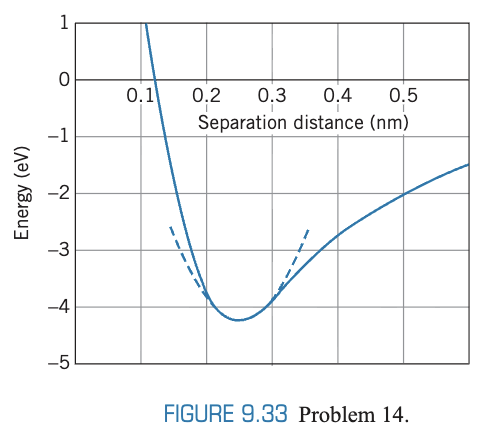
\includegraphics[width=0.35\textwidth]{image-9-14.png} 
            % \label{fig:wrapfig}
        \end{wrapfigure}
        Figure 9.33 shows the energy minimum of molecular \ce{NaCl}, through which a parabola has been drawn. 
        Following the methods of Example 9.3, find (a) the effective vibrational force constant, (b) the vibrational frequency and (c) wavelength, and (d) the vibrational photon energy for \ce{NaCl}. 
        (e) In what range of the electromagnetic spectrum would such radiations be found? 
        (f) What is the maximum vibrational quantum number for which the parabolic approximation remains valid for \ce{NaCl}?

        \subsubsection{Solution (a)}
            At the points designated, the difference in distance is about $0.08\,\unit{\nano\meter}$.
            The depth diffference it reaches is about $0.2\,\unit{\eV}$.
            We can plug this into an equation used in 9.3.
            \begin{align}
                k   &=  \frac{2(\Delta E)}{(\Delta R)^2}
                    =   \frac{0.4\,\unit{\eV}}{0.0064\E{-18}\,\unit{\meter^2}}
                    =   \boxed{62.5\E{18}\,\unit{\eV/\meter^2}}
            \end{align}

        \subsubsection{Solution (b)}
            Find the effective mass.
            \begin{equation}
                m   =   \frac{22.99 * 35.45}{22.99 + 35.45}
                    =   \frac{814.9955}{58.44}
                    =   13.95
            \end{equation}

            Plug this into an equation for the frequency.
            \begin{align}
                f   &=  \frac{1}{2\pi} \sqrt{\frac{kc^2}{mc^2}}
                    =   \frac{1}{2\pi} \sqrt{\frac{(62.5\E{18}\,\unit{\eV/\meter^2})(2.998\E{8}\,\unit{\meter/\second})^2}{(13.95\,\unit{\amu})(931.5\E{6}\,\unit{\eV/\amu})}}\\
                    &=  \frac{1}{2\pi} * 20.8\E{12}\,\unit{\hertz}
                    =   \boxed{3.31\E{12}\,\unit{\hertz}}
            \end{align}

        \subsubsection{Solution (c)}
            Use $c = \lambda f$.
            \begin{equation}
                \lambda = \frac{c}{f}
                    =   \frac{2.998\E{8}\,\unit{\meter/\second}}{3.31\E{12}\,\unit{\hertz}}
                    =   \boxed{90.6\,\unit{\micro\meter}}
            \end{equation}

        \subsubsection{Solution (d)}
            \begin{align}
                E   &=  hf
                    =   6.626\E{-34}\,\unit{\joule\cdot\second} \cdot 3.31\E{12}\,\unit{\hertz}\\
                    &=  \boxed{2.19\E{-21}\,\unit{\joule}}
                    =   0.01366891\,\unit{\eV}
            \end{align}

        \subsubsection{Solution (e)}
            These are microwaves, so you could warm up your lunch with it.

        \subsubsection{Solution (f)}
            Knowing the maximum of $0.4\,\unit{\eV}$, divide it by the energy of one photon that would be released.
            \begin{equation}
                n   =   \frac{0.4}{0.01366891}
                    =   29.26
            \end{equation}

            Round this down to the nearest $N + \frac{1}{2}$, and we get $28.5$.
            This means that the maximum value of $N$ is \boxed{28}.
            
        
    \pagebreak
    \subsection{Problem 17}
        Following the method of Example 9.4, calculate the energies and wavelengths of the three lowest rotational transitions emitted by molecular \ce{NaCl}. 
        In what region of the electromagnetic spectrum would these radiations be found?

        \subsubsection{Solution}
            First, find the effective mass.
            \begin{equation}
                m   =   \frac{22.99 * 35.45}{22.99 + 35.45}
                    =   \frac{814.9955}{58.44}
                    =   13.95\,\unit{\amu}
            \end{equation}

            Then, find the separation distance.
            Based on the graph in Figure 9.33, my estimate for the separation at equilibrium is $0.25\,\unit{\nano\meter}$.
            Plug this in to what the textbook calls the rotational quantity $B$.
            \begin{align}
                B   &=  \frac{\hbar^2 c^2}{2mc^2R_{\rm eq}^2}
                    =   \frac{(197.3\,\unit{\eV\cdot\nano\meter})^2}{2(13.95\,\unit{\amu})(931.5\,\unit{\mega\eV/\amu})(0.25\,\unit{\nano\meter})^2}\\
                    &=  23.97\E{-6}\,\unit{\eV}
            \end{align}

            From here, multiply it by 2, 4, and 6 to ge the three lowest transitions ($n = 2B(L+1)$).
            \begin{align}
                n = 1 \to E = 47.93\E{-6}\,\unit{\eV} \to \lambda = 25.87\,\unit{\milli\meter}\\
                n = 2 \to E = 95.86\E{-6}\,\unit{\eV} \to \lambda = 12.94\,\unit{\milli\meter}\\
                n = 3 \to E = 143.8\E{-6}\,\unit{\eV} \to \lambda = 8.623\,\unit{\milli\meter}
            \end{align}

            These would be the radar waves, or maybe longer microwaves.
        
\pagebreak
\section{Chapter 10}
    \subsection{Question 5}
        How is the speed distribution of a gas at temperature $T$ different from that at temperature $2T$? 
        The energy distribution? 
        Sketch the speed and energy distributions at the two temperatures.

        \subsubsection{Answer}
            Here is the Maxwell Speed Distribution.
            \begin{equation}
                N(v) = N \sqrt{\frac{2}{\pi}} \left( \frac{m}{kT} \right)^{3/2} v^2 \e{-\frac{mv^2}{2kT}}
            \end{equation}

            Replace $T$ with $2T$.
            \begin{align}
                N(v)    &=  N \sqrt{\frac{2}{\pi}} \left( \frac{m}{k2T} \right)^{3/2} v^2 \e{-\frac{mv^2}{2k2T}}\\
                    &=  N \sqrt{\frac{2}{\pi}} \left( \frac{m}{kT} \right)^{3/2} * \frac{1}{2^{3/2}} v^2 \e{-\frac{mv^2}{2kT} + \frac{mv^2}{4kT}}\\
                    &=  N \sqrt{\frac{2}{\pi}} \left( \frac{m}{kT} \right)^{3/2} v^2 \e{-\frac{mv^2}{2kT}} * \frac{\e{\frac{mv^2}{4kT}}}{2^{3/2}}
                    =   N(v) * \frac{\e{\frac{mv^2}{4kT}}}{2^{3/2}}
            \end{align}

            Where $\e{\frac{mv^2}{4kT}} > 2^{3/2}$, it amplifies upwards, while in the opposite, it amplifies downwards.
            This would give the appearance of the velocity curve move its mean to the right but extending its deviation wider.
    
    \pagebreak
    \subsection{Question 11}
        Estimate the mean kinetic energy of the ``free'' electrons in a metal if they obeyed Maxwell-Boltzmann statistics. 
        How does this compare with the result of applying Fermi-Dirac statistics? 
        Why is there such a difference?

        \subsubsection{Answer}
            For the mean, the, we use $f(E)$ and $g(E)$. 
            \begin{gather}
                dN = N(E)\,dE = V g(E) f(E)\,dE\\
                \begin{align}
                    \left\langle E \right\rangle    &=  \int_{0}^{\infty} \frac{E * N(E)}{N}\,dE
                        =   \int_{0}^{\infty} \frac{E * V g(E) f(E)}{N}\,dE\\
                        &=  \frac{V}{N} \int_{0}^{\infty} E g(E) f(E)\,dE
                        =   \frac{V}{N} \int_{0}^{\infty} \frac{8 \pi \sqrt{2} m^{3/2}}{h^3} E^{3/2} f(E)\,dE\\
                        &=  \frac{8 V \pi \sqrt{2} m^{3/2}}{h^3 N} \int_{0}^{\infty} E^{3/2} f(E)\,dE
                \end{align}
            \end{gather}

            For the Boltzmann distribution, we get the below, from conference.
            \begin{equation}
                \left\langle E \right\rangle = \frac{3}{2} k_B T
            \end{equation}

            Now for Fermi-Dirac.
            \begin{align}
                \left\langle E \right\rangle    &=  \frac{8 V \pi \sqrt{2} m^{3/2}}{h^3 N} \int_{0}^{\infty} \frac{E^{3/2}}{\e{(E-E_F)/kT} + 1} \,dE
            \end{align}
            
            This is a very complicated integral. 
            At zero or near zero temperatures, the energy would be the following equation.
            \begin{equation}
                \left\langle E \right\rangle = \frac{3 h^2}{10 m} \left( \frac{3N}{8\pi V} \right)^{2/3}
            \end{equation}

            However, at near zero temperature, Maxwell-Boltzmann would estimate the mean energy to be even closer to zero.
            This is because the Maxwell-Boltzmann equation approaches zero as $T$ approaches 0, while the Fermi-Dirac does not.
        
    \pagebreak
    \subsection{Problem 2}
        (a) Considering the numbers of heads and tails, how many macrostates are there when 5 coins are tossed? 
        (b) What is the total number of possible microstates in tossing 5 coins?
        (c) Find the number of microstates for each macrostate, and be sure the total agrees with your answer to part (b).

        \subsubsection{Solution (a)}
            There are \underline{six} possible states.\\
            \begin{tabular}{| c | c | c | c | c | c | c |}
                \hline
                State   &   1   &   2   &   3   &   4   &   5   &   6\\ \hline
                Heads   &   0   &   1   &   2   &   3   &   4   &   5\\ \hline
                Tails   &   5   &   4   &   3   &   2   &   1   &   0\\
                \hline
            \end{tabular}

        \subsubsection{Solution (b)}
            Since there are two possible states per coin and five coins, the number of total microstates is $2^5 = \boxed{32}$.

        \subsubsection{Solution (c)}
            This is classical probability (n choose k).
            \begin{equation}
                W_N =   \binom{5}{N}    =   \frac{5!}{k!(5-k)!}
            \end{equation}
            \begin{multicols}{2}
                \begin{align}
                    W_0 &=  \binom{5}{0}    =   \frac{5!}{0!5!} =   1\\
                    W_1 &=  \binom{5}{1}    =   \frac{5!}{1!4!} =   5\\
                    W_2 &=  \binom{5}{2}    =   \frac{5!}{2!3!} =   10
                \end{align}

                \begin{align}
                    W_3 &=  \binom{5}{3}    =   \frac{5!}{3!2!} =   10\\
                    W_4 &=  \binom{5}{4}    =   \frac{5!}{4!1!} =   5\\
                    W_5 &=  \binom{5}{5}    =   \frac{5!}{5!0!} =   1
                \end{align}
            \end{multicols}

            The total is still 32.
            
        
    \pagebreak
    \subsection{Problem 6}
        A system of four oscillator-like particles shares 8 units of energy. 
        (That is, the particles can accept energy only in equal units, in which the oscillator spacing is 1 unit.)
        (a) List the macrostates, and for each macrostate give the number of microstates for distinguishable classical particles, indistinguishable quantum particles with integral spin, and indistinguishable quantum particles with half-integral spin.
        (b) Calculate the probability to find a particle with exactly 2 units of energy for each of the three different types of particles.

        \subsubsection{Solution (a)}
            \begin{wrapfigure}{r}{0.5\textwidth}
                \vspace{-30pt}
                \tiny
                \begin{flushright}
                    \begin{tabular}{| c | c | c | c | c | c | c | c |} \hline
                        State   &1  &2  &3  &4  &$W$    &$W_{\mathbb{N}_0}$ &$W_{\mathbb{N}_0 + \frac{1}{2}}$\\ \hline
                        1       &8  &0  &0  &0  &4      &1                  &0\\
                        2       &7  &1  &0  &0  &12     &1                  &1\\
                        3       &6  &2  &0  &0  &12     &1                  &1\\
                        4       &6  &1  &1  &0  &12     &1                  &1\\
                        5       &5  &3  &0  &0  &12     &1                  &1\\
                        6       &5  &2  &1  &0  &24     &1                  &1\\
                        7       &5  &1  &1  &1  &4      &1                  &0\\
                        8       &4  &4  &0  &0  &6      &1                  &1\\
                        9       &4  &3  &1  &0  &24     &1                  &1\\
                        10      &4  &2  &2  &0  &12     &1                  &1\\
                        11      &4  &2  &1  &1  &12     &1                  &1\\
                        12      &3  &3  &2  &0  &12     &1                  &1\\
                        13      &3  &3  &1  &1  &6      &1                  &1\\
                        14      &3  &2  &2  &1  &12     &1                  &1\\
                        15      &2  &2  &2  &2  &1      &1                  &0\\ \hline
                        Total   &   &   &   &   &165    &15                 &12\\ \hline
                    \end{tabular}
                \end{flushright}
                % \caption{Table of Configurations}
            \end{wrapfigure}
            My configurations are on the right. 
            My total number of macrostates is 15.
            The number of microstates for each macrostate can be calculated with equation (\ref{eq:2.4.a.1}).
            \begin{equation}
                \label{eq:2.4.a.1}
                W = \frac{N!}{\prod_{i=0}^8 N_i !}
            \end{equation}

            The value of $N$ is 4.
            The value of $N_i$ is the number of particles with energy level $i$.
            For integral spin quantum particles, the value of $W_{\mathbb{N}_0}$ is always 1.
            For half-integral spin quantum particles, the value of $W_{\mathbb{N}_0 + \frac{1}{2}}$ is 0 when more than 2 particles have the same energy level and 1 otherwise.

        \subsubsection{Solution (b)}
            In all three cases, we will be using equation (\ref{eq:2.4.b.1}).
            \begin{equation}
                \label{eq:2.4.b.1}
                p(E) = \frac{\sum_{i=0}^{8} N_i W_i}{N \sum_{i = 0}^{8} W_i}
            \end{equation}
            
            $N_i$ is the number of particles of energy $E$ in the configuration $i$.

            \paragraph{Distinguishable Classical Particles}
                Use $W$ from the table for $W$. 
                Set $E = 2$.
                
                \begin{align}
                    \begin{split}
                        \sum N_i W_i    &= 0*4 + 0*12 + 1*12 + 0*12 + 0*12 + 1*24 \\
                                        &\quad + 0*4 + 0*6 + 0*24 + 2*12 + 1*12 + 1*12\\ 
                                        &\quad + 0*6 + 2*12 + 4*1 = 88
                    \end{split}\\
                    p(2)    &=  \frac{88}{8*165}
                            =   \frac{11}{165}
                            =   \boxed{\frac{1}{15} \approx 0.0667}
                \end{align}

            \paragraph{Indistinguishable Integer Spin Particles}
                Use $W_{\mathbb{N}_0}$ from the table for $W$. 
                Set $E = 2$.
                All values of W are 1.
                
                \begin{align}
                    \begin{split}
                        \sum N_i W_i    &= 0*1 + 0*1 + 1*1 + 0*1 + 0*1 + 1*1 \\
                                        &\quad + 0*1 + 0*1 + 0*1 + 2*1 + 1*1 + 1*1\\ 
                                        &\quad + 0*1 + 2*1 + 4*1 = 10
                    \end{split}\\
                    p(2)    &=  \frac{10}{8*15}
                            =   \boxed{\frac{1}{12} \approx 0.0833}
                \end{align}

            \paragraph{Indistinguishable Half-Integer Spin Particles}
                Use $W_{\mathbb{N}_0 + \frac{1}{2}}$ from the table for $W$. 
                Set $E = 2$.
                All values of W are 1.
                
                \begin{align}
                    \begin{split}
                        \sum N_i W_i    &= 0*0 + 0*1 + 1*1 + 0*1 + 0*1 + 1*1 \\
                                        &\quad + 0*0 + 0*1 + 0*1 + 2*1 + 1*1 + 1*1\\ 
                                        &\quad + 0*1 + 2*1 + 4*0 = 8
                    \end{split}\\
                    p(2)    &=  \frac{8}{8*12}
                            =   \boxed{\frac{1}{12} \approx 0.0833}
                \end{align}
        
    \pagebreak
    \subsection{Problem 10}
        Calculate the density of states (per unit area) for a collection of photons confined to a two-dimensional region in the shape of a square a length L on each side.

        \subsubsection{Solution}
            As in the textbook, we begin with $E = pc$.
            Also take the derivative with respect to $n$.
            \begin{align}
                E   &=  |p|c
                    =   \frac{\hbar c \pi}{L} \left| \vec{n} \right| \to n = \frac{L}{\hbar c \pi} E\\
                dE  &=  \frac{\hbar c \pi}{L}\,dn \to dn = \frac{L}{\hbar c \pi}\,dE
            \end{align}

            Find the differential of the area of a circle with respect to radius $n$.
            Only consider one quadrant.
            \begin{gather}
                A = \frac{1}{4}(\pi n^2) = \frac{\pi}{4} \frac{L^2}{\hbar^2 c^2 \pi^2} E^2\\
                \diff{A}{n} = \frac{1}{4} \diff{}{n} \pi n^2 = \frac{\pi}{2} n\\
                dA = dN = \frac{\pi}{2} n\,dn = A \cdot g(n)\,dn
            \end{gather}

            Photons have only two polarizations that we can consider, so we can multiply it by two.
            \begin{equation}
                dA = A \cdot g(n)\,dn = \pi n\,dn
            \end{equation}

            From here, plug in the values of $n(E)$ and use the equation of the density of states.
            \begin{align}
                dN  &=  dA
                    =   \pi n\,dn
                    =   \pi \left( \frac{L}{\hbar c \pi} E \right) \left( \frac{L}{\hbar c \pi}\,dE \right)
                    =   \frac{L^2}{\hbar^2 c^2 \pi} E\,dE\\
                g(E)    &=  \diff{N}{E}
                    =   \frac{L^2}{\hbar^2 c^2 \pi} E
            \end{align}

            Dividing this by the area of the box ($L^2$), we can find the density per unit area.
            \begin{equation}
                \frac{g(E)}{L^2} = \boxed{\frac{E}{\hbar^2 c^2 \pi}}
            \end{equation}
        
    \pagebreak
    \subsection{Problem 15}
        A container holds one mole of helium gas at a temperature of 293 K.
        (a) Show that the mean energy $E_m$ of the molecules is 0.0379 eV.
        (b) How many molecules have energies in an interval of width $0.01E_m$ centered on $E_m$ ?

        \subsubsection{Solution (a)}
            In conference, we derived an equation for the average energy from the temperature.
            \begin{align}
                \left\langle E \right\rangle
                    &=  \frac{3}{2} k_B T
                    =   \frac{3}{2} * 1.38\E{-23}\,\unit{\joule/\kelvin} * 293\,\unit{\kelvin}\\
                    &=  6.0651\E{-21}\,\unit{\joule} * \frac{1\,\unit{\eV}}{1.602\E{-19}\,\unit{\joule}}\\
                    &=  0.0378596\,\unit{\eV}
                    \approx \boxed{0.0379\,\unit{\eV}}
            \end{align}

        \subsubsection{Solution (b)}
            \begin{align}
                N(E)    &=  \frac{2N}{\sqrt{\pi} (k_B T)^{3/2}} E^{1/2} \e{-E/k_B T}\\
                \frac{dN}{N}    &=  \frac{N(E)\,dE}{N}    =   \frac{2}{\sqrt{\pi} (k_B T)^{3/2}} E^{1/2} \e{-E/k_B T}\,dE\\
                    &=  \frac{2}{\sqrt{\pi} (k_B T)^{3/2}} E^{1/2} \e{-E/k_B T}\,dE
            \end{align}

            Here, we use $E = E_m$ and $dE = 0.01 E_m$.
            \begin{align}
                \frac{dN}{N}    &=  \frac{0.01 * 2}{\sqrt{\pi} (0.0252)^{3/2}} E_m^{3/2} e^{-E_m/0.0252}
                    =   0.0046254
            \end{align}

            Multiply both sides by the number of molecules ($N_A$ in this case) to get the answer.
            \begin{equation}
                N_A * 0.0046254 =   \boxed{2.78542\E{21}}
            \end{equation}
        
    \pagebreak
    \subsection{Problem 21}
        A blackbody is radiating at a temperature of $2.50\E{3}\,\unit{\kelvin}$.
        (a) What is the total energy density of the radiation? 
        (b) What fraction of the energy is emitted in the interval between 1.00 and 1.05 eV? 
        (c) What fraction is emitted between 10.00 and 10.05 eV?

        \subsubsection{Solution (a)}
            Blackbody comes from Bose-Einstein.
            The energy energy distribution function of the Bose-Einstein is below.
            \begin{equation}
                f_{BE}(E) = \frac{1}{A_{BE}\e{E/kT} - 1}
            \end{equation}

            Looking at the textbook, we can find a formula for the energy density from thermal radiation.
            \begin{equation}
                U   =   \frac{8\pi^5 k_B^4}{15(hc)^3} T^4
            \end{equation}

            Plug in values here to find the energy density.
            \begin{align}
                U   &=  \frac{8\pi^5 (8.617\E{-5}\,\unit{\eV/\kelvin})^4}{15(1240\,\unit{\eV\cdot\nano\meter})^3} (2.50\E{3}\,\unit{\kelvin})^4\\
                    &=  \boxed{1.8436\E{-10}\,\unit{\eV/\nano\meter^3}}
            \end{align}

        \subsubsection{Solution (b)}
        Blackbody ratation is photons, so use that for $g(E)$.
            \begin{align}
                g(E)    &=  \frac{8\pi}{(hc)^3}E^2\\
                U(E)\,dE    &=  E g(E) f(E)\,dE
                    =   \frac{8\pi}{(hc)^3}E^3 \frac{1}{\e{E/kT} - 1}\,dE\\
            \end{align}

            Set $E_1 = 1.00$ and $E_2 = 1.05$.
            Take a fraction to find the total fraction.
            We integrate it on top over the area specified and on bottom over the entire positive axis.
            \begin{align}
                R   &=  \frac{\int_{1.00}^{1.05}\frac{E^3}{\e{E/kT} - 1}\,dE}{\int_{0}^{\infty}\frac{E^3}{\e{E/kT} - 1}\,dE}
            \end{align}

            The bottom integral has the value of $(kT)^4\frac{\pi^4}{15}$.
            \begin{equation}
                R = (kT)^{-4} \frac{15}{\pi^4} \int_{1.00}^{1.05}\frac{E^3}{\e{E/kT} - 1}\,dE
            \end{equation}

            The top half of the fraction is very difficult to compute. 
            Since the midpoint approximation exists, I'll do that instead.
            \begin{align}
                R   &=  (0.215)^{-4} \frac{15}{\pi^4} \frac{1.025^3}{\e{1.025/0.215} - 1} * 0.05
                    =   \boxed{0.033}
            \end{align}

        \subsubsection{Solution (c)}
            Same equation.
            \begin{align}
                R   &=  (0.215)^{-4} \frac{15}{\pi^4} \frac{10.025^3}{\e{10.025/0.215} - 1} * 0.05
                    =   \boxed{2.2\E{-17}}
            \end{align}
        
    \pagebreak
    \subsection{Problem 23}
        Compute the Fermi energy and the average electron energy for copper.

        \subsubsection{Solution}
            First find the number of electrons per unit volume.
            \begin{align}
                \frac{N}{V} &=  \frac{\rho N_A}{M}
                    =   \frac{(8960\,\unit{\kilo\gram/\meter^3})(6.022\E{23}\,\unit{\mole^{-1}})}{0.06355\,\unit{\kilo\gram/\mole}}
                    =   8.49\E{28}\,\unit{\meter^{-3}}
            \end{align}

            Now use the formula for the Fermi energy.
            \begin{align}
                E_F &=  \frac{h^2}{2m} \left( \frac{3}{8\pi} \frac{N}{V} \right)^{2/3}
                    =   \frac{(1240\,\unit{\eV\cdot\nano\meter})^2}{2(0.511\E{6}\,\unit{\eV})} \left( \frac{3}{8\pi} 8.49\E{28}\,\unit{\meter^{-3}} \right)^{2/3}\\
                    &=  \boxed{7.046\,\unit{\eV}}
            \end{align}

            The average electron energy is calculated using a different formula.
            \begin{equation}
                E_m =   \frac{3}{5} E_F
                    =   \frac{3}{5} 7.046\,\unit{\eV}
                    =   \boxed{4.227\,\unit{\eV}}
            \end{equation}
        
    \pagebreak
    \subsection{Problem 25}
            A certain metal has a Fermi energy of 3.00 eV. 
            Find the number of electrons per unit volume with energy between 5.00 eV and 5.10 eV for (a) $T = 295\,\unit{\kelvin}$; (b) $T = 2500\,\unit{\kelvin}$.

            \subsubsection{Solution (a)}
                I'll be using an estimation again, since this involves a pretty nasty integral.
                \begin{align}
                    \frac{N}{V} &=  \frac{8\pi\sqrt{2}m^{3/2}}{h^3} \int_{5.00\,\unit{\eV}}^{5.10\,\unit{\eV}} \frac{E^{1/2}}{\e{(E - E_F)/kT} + 1}\,dE\\
                        &\approx    \frac{8\pi\sqrt{2}(0.511\E{6})^{3/2}}{(1240\E{-9})^3} * \frac{(5.05\,\unit{\eV})^{1/2}}{\e{(5.05\,\unit{\eV} - 3.00\,\unit{\eV})/kT} + 1} * 0.10\,\unit{\eV}\\
                        &=  \boxed{4.649\E{-14}\,\unit{\meter^{-3}}}
                \end{align}

            \subsubsection{Solution (b)}
                \begin{align}
                    \frac{N}{V} &\approx    \frac{8\pi\sqrt{2}(0.511\E{6})^{3/2}}{(1240\E{-9})^3} * \frac{(5.05\,\unit{\eV})^{1/2}}{\e{(5.05\,\unit{\eV} - 3.00\,\unit{\eV})/kT} + 1} * 0.10\,\unit{\eV}\\
                        &=  \boxed{1.127\E{23}\,\unit{\meter^{-3}}}
                \end{align}
\end{document}